% This is samplepaper.tex, a sample chapter demonstrating the
% LLNCS macro package for Springer Computer Science proceedings;
% Version 2.20 of 2017/10/04
%
\documentclass[runningheads]{llncs}
%
\usepackage{graphicx}
% Used for displaying a sample figure. If possible, figure files should
% be included in EPS format.
%
% If you use the hyperref package, please uncomment the following line
% to display URLs in blue roman font according to Springer's eBook style:
% \renewcommand\UrlFont{\color{blue}\rmfamily}

\begin{document}
%
\title{ScSpark: Low-Redundancy disk access and High-Performance tool for the Single-Cell RNA sequenccing data processing\thanks{Supported by organization x.}}
%
%\titlerunning{Abbreviated paper title}
% If the paper title is too long for the running head, you can set
% an abbreviated paper title here
%
\author{First Author\inst{1}\orcidID{0000-1111-2222-3333} \and
Second Author\inst{2,3}\orcidID{1111-2222-3333-4444} \and
Third Author\inst{3}\orcidID{2222--3333-4444-5555}}
%
\authorrunning{F. Author et al.}
% First names are abbreviated in the running head.
% If there are more than two authors, 'et al.' is used.
%
\institute{Princeton University, Princeton NJ 08544, USA \and
Springer Heidelberg, Tiergartenstr. 17, 69121 Heidelberg, Germany
\email{lncs@springer.com}\\
\url{http://www.springer.com/gp/computer-science/lncs} \and
ABC Institute, Rupert-Karls-University Heidelberg, Heidelberg, Germany\\
\email{\{abc,lncs\}@uni-heidelberg.de}}
%
\maketitle
%
\begin{abstract}
High-throughput single-cell RNA sequencing
  (scRNA-seq) data processing pipelines use multiple steps to transform raw barcode next-generation sequencing(NGS) data to express matrices, including sequence quality control, genome alignment and transcript counting.
However, with the incresasing of scRNA-seq data volume, file input/output(IO) becomes the bottleneck of pipeline performance.
We take advantage of Spark's in-memory computing and scalable trait to develop a new Java-based program called ScSpark.
ScSpark can distribute scRNA-seq data processing tasks in the cluster and can elminate all disk accessing for intermediate results.
We combine Spark and our proposed function to implement sequence quality control and transcript counting.
Furthermore, we choose STAR as our aligner.
In order to avoid unneccessary disk accessing while reading FASTQ file and writing SAM file, we use Java Native Interface(JNI) to deliver FASTQ RDD to invoke STAR, and then transform return value to SAM RDD.
We use peripheral blood mononuclear cell(PBMC)\_10k\_v3 as our dataset and build spark's cluster on Aliyun to test ScSpark.
The experiment results indicates ScSpark faster and more scalable than any tradition pipelines.
\keywords{Intermediate Data \and Fast \and Scalable.}
\end{abstract}

\section{Introduction}
In recent years, new molecular biology technologies based on second-generation sequencing have emerged one after another.
However, current conventional sequencing methods can only analyze the cell population.
And the final difference is the average difference of the cell population.
But from a molecular point of view, human cells are not exactly the same, there are differences between cells~\cite{Papalexi2018SinglecellRS}.
In this context, single cell sequencing is very important.
Single-cell sequencing not only reveals unique changes in each cell, but also enables the discovery of entirely new cell types, greatly facilitating genomics, enabling precise differentiation of cell types and enabling researchers to study molecular mechanisms at the single-cell level.
ScRNA-seq is a widely used single-cell sequencing at present, which is achieved through reverse transcription, amplification, and sequencing of all RNA from a single cell, followed by relevant bioinformatics analysis. 
The large
         -scale 
                scRNA-seq technology represented by 10X Genomics is becoming one of the most prevalent platforms.

The introduction of cell barcode(CB), which assigns different sequences to each cell for transcriptional source retrieval after sequencing, greatly increases the total length of sequencing and reduces the cost of scRNA-seq~\cite{Macosko2015HighlyPG}~\cite{Klein2015DropletBF}.
These barcodes allow reads to be multiplexed after the cells have been assembled for sequencing.~\cite{tian2018scPipe}.
Apart from cellular barcodes, Unique Molecular Identifiers(UMIs) are random oligonucleotide barcodes that are used in high-throughput sequencing experiments\cite{Kivioja2012Counting}~\cite{camara2017Methods}.
By UMI, the same copy from different molecules and the same copy from the same molecule for PCR amplification could be distinguished. ~\cite{smith2017UMI}.

In the scRNA-seq experiment, the use of multi-level barcodes presented additional challenges for data processing, which was quite different from the traditional bulk RNA-seq and low-throughput scRNA-seq experiments.
In recent years, researchers have developed multiple scRNA-seq data processing pipelines, typically implementing steps including sequence quality control, genome alignment, and transcript counting to convert raw scRNA-seq data into an expression matrix for further downstream analysis.
The first step is to filter fastq readings with low quality BC based on user-defined thresholds.
This step eliminates most of the false CBs, greatly improving the accuracy of the CBs that need to be considered for counting, while eliminating the low-quality UMI.
The remaining fastq reads are then mapped to genomes using the splice-aware aligner, such as STAR~\cite{dobin2012RNA} or HISAT2~\cite{kim2015hisat}.
Next, reads are assigned to genes and then generate count tables for UMIs and reads per gene per CB~\cite{swati0zUMIs}.

Nowadays, there are many tools to deal with scRNA-seq, among which the most popular ones are CellRanger~\cite{zheng2017Massively}, umis~\cite{Svensson2017PowerAO}, dropEst~\cite{Petukhov2018dropEstPF}, zUMIs~\cite{swati0zUMIs}, Drop-seq tools~\cite{Macosko2015HighlyPG}, scPipe~\cite{tian2018scPipe} and UMI-tools~\cite{Smith2017UMItoolsMS}~\cite{gao2020Comparison}. 
UMI-tools~\cite{ref_url1} is an open source tool with an impressive clear process, Our ScSpark is based on improvements to this tool.
CellRanger which is a highly integrated data process software tailored by 10X Genomics for single-cell RNA sequencing analysis and it performs comparatively well on machine with enough CPU and memory resources in the big data set, but did badly in small data set.
STARsolo~\cite{2019STARsolo} has improved the parallelism of sequence mapping and counting procedures, and achieved good performance on a single machine.
It is a pity that all tradition pipeline cannot be extended to multiple nodes.

There have been many studies using big data framework like 
                                                           Hadoop~\cite{ref_url2}
                                                                                  and Spark~\cite{ref_url3} to optimize biological data processing.
Due to more efficiency in utilizing memory computing, Spark is a better big data computing framework than Hadoop's MapReduce~\cite{dean2008mapreduce}~\cite{zaharia2012resilient}.
SparkBWA~\cite{abuin2016sparkbwa} and GPF~\cite{li2018high} are good frameworks that both improve the efficiency of DNA sequencing upstream data processing by Spark.
Falco~\cite{Yang2016Falco} has tried to use Spark in scRNA-seq upstream data processing.
However, its flexibility was limited to a shallow reworking of the pipeline consisting of two popular RNA-seq alignment/feature quantification tools and no consideration of scRNA-seq data features(such as UMI and CB).
And processing for UMI and CB are the most time-consuming steps in scRNA-seq pipelines.
Second, Falco's Implementation way depends on tradition pipeline's tool which'll cause low parallelism in each node's internal.
Most important, Falco’s operations have lots of redundancy disk access which causes it doesn't utilize Spark’s in-memory compute advantage well.

To more efficient use Spark's parallel and in memory compute advantage, we totally use Spark's function to implement sequence quality control but not like Falco use tradition pipeline.
And different with Falco, we enhance STAR's file IO interface, to reduce redundant disk access.
In the end, scSpark has implemented transcript counting by combining Spark function and our algorithm to achieve parallel compute.
The traditional single machine serial processing mode has been unable to meet the demand of computing and storage resources for super-large scale scRNA-seq data.
Our work plans to adopt Spark system architecture propose a set of in memory computing and scalable scRNA-seq data processing pipeline, which can significantly reduce the processing time.

\section{Method}
\subsection{Overview}
We implemented our program based on the Spark framework to utilize Spark's advantage, run program across the cluster, and default cache data keeps in memory.
With the increasing of dataset volume, the time to process intermediate result file occupies a more significant proportion on total time.
And the single machine's capacity is not sufficient to adapt the increasing scRNA-seq data volume.
Therefore, reducing the disk access of intermediate result file and improving the upstream data process's scalability is our scSpark's target.

\subsection{Spark Version Filter}
\begin{figure}
  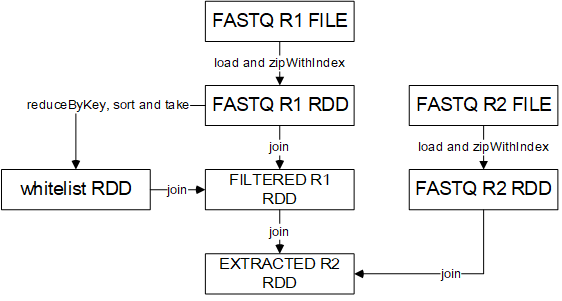
\includegraphics[width=\textwidth]{fig1.png}
  \caption{An overview of Spark version filter.} \label{fig1}
\end{figure}  
Large FASTQ file can load in each node's memory parallel therefore the load speed doesn't limit by single node disk access speed.
As shown in Fig~\ref{fig1}, the filter step typically consists of two main components, generate whitelist which can identity of the true cell barcodes is unknown, use the whitelist to filter FASTQ R1 and then extract FASTQ R2 according to filtered FASTQ R1's index.

We load each split of FASTQ R1 to memory, and abstract them as FASTQ R1 RDD.
Generate whitelist actually is a top N problem that the problem can use Spark's function to achieve parllel compute.
By using reduceByKey function, FASTQ R1 RDD can count each split's barcodes times parallel and sum each split's result in the end.
After that we can use the result to generate whitelist RDD by Spark's sort and take function, both can parallel compute in the cluster.
We can easily get filtered FASTQ R1 RDD, by using the join function to find which read's cell barcode is in the whitelist.
The last step in filter is extracting FASTQ R2.
We use the join function again to combine filtered FASTQ R1 RDD and FASTQ R2 RDD with the same index.
\subsection{Eleminate redundancy disk access in Aligner step}
\begin{figure}
  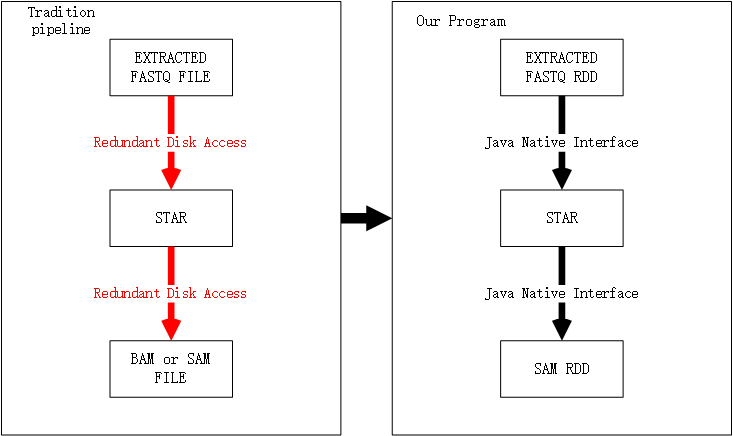
\includegraphics[width=\textwidth]{fig2.png}
  \caption{New way to implement STAR's interface.} \label{fig2}
\end{figure}
Apart from Cellranger we can't know how it implements because it isn't a open source software, in tradition pipeline, STAR need load extracted Fastq R2 file or load Fastq R1, R2 and whitelist actually will generate unneccessary disk access.  
We choose STAR as our aligner but modify how STAR loads FASTQ file to avoid load extracted FASTQ R2 and FASTQ R1 twice. 
As shown in Fig~\ref{fig2}, we utilize Java Native Interface to transfer extracted FASTQ R2 RDD's data to STAR, and then start the STAR process.
To overcome node's data volume imbalance problem, we repartition the extracted FASTQ R2 RDD, and then each node can run STAR parallel and with counterpoise data volume.
We also find if node's in memory is enough, we can start up more than one STAR's in one node to achieve better parallel.
STAR's result SAM or BAM file generate more disk access waste than STAR's input, we refer STAR-solo's solution to solve the problem by combining aligner and count.
We use Java Native Interface again to transfer STAR result and directly abstract them to SAM RDD.
This operation is parallel and totally in memory.

\subsection{Count with multi-node}
\begin{figure}
  \centering
  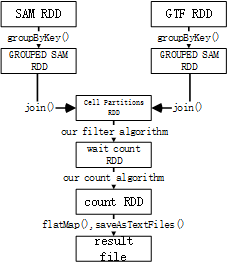
\includegraphics{fig3.png}
  \caption{An overview of Spark version count.} \label{fig3}
\end{figure}
As shown in Fig~\ref{fig3}, to take advantage multi-node's compute capability, we use a new way to implement count step.
Except SAM RDD that generate in the previous step, we load GTF file to memory and abstract them as GTF RDD.
Then we group SAM RDD and GTF RDD by their cell name and due to different cell's record can't influence the other's count, we use flatMap to parallel compute each cell's read count.
In the end, we collect result in all nodes, and the result file will produce the only output disk access in the whole program.
ScSpark breaks the limitation of one node's compute and can scale easily.

\section{Results}
We'll evaluate the speed, scalabilty and compare each step's scalability of our program in this section.
First, we'll run our program and tradition pipeline and use process time to evaluated the advantage of scSpark.
And then, the index of speedup helps us to examify the scalability of scSpark.
In the end, we compare each step's scalability to find the reason why scSpark's scalability also has a ceiling.
\subsection{Experiment environments and Data Sets prepare}
We use Apache Spark version 2.1.0 as our in-memory computing environment.
The Spark cluster consists of Aliyun's ECS, and each node consists of 16 vCPU
(Intel Xeon(Cascade Lake) Platinum 8269CY at 2.5GHz), 128 GBytes of DRAM and 400 GBits ESSD.

An example scRNA-seq dataset generated by 10X Genomics on their platform was used in our experiments.
10X-PBMC-10k dataset: 10X Genomics v3 10k peripheral blood mononuclear cell (PBMC) from a healthy donor~\cite{ref_url4}. 
It contains two gzipped FASTQ files, after unzip, FASTQ R1's volume is 69 Gbytes, and FASTQ R2's volume is 144 Gbytes, each of that file contain 640 millions records.
We used STAR as our aligner, mapping to an index built on the human NCBI38 reference which called GRCh38.p12.genome.fa and use genome.gtf~\cite{ref_url5} to filter the SAM~\cite{ref_url5}.
To evaluate the reason of why scSpark have a scalability ceiling and to experiment more convenient, we split FASTQ file to 100 millions, 160 millions and 320 millions records,.
\subsection{Efficiency Evaluation}
\begin{table}
  \centering
  \caption{tradition pipelien and scSpark's performance compare}\label{tab1}
  \begin{tabular}{l | l | l  l}
  \hline
  System &  Cores & Data volume size(s) \\
  \hline
   &  & 100 million(reads) & 640 million(reads) \\
  \hline
  UMI-tools & 64 cores & 7254 & 44160 \\
  \hline
  CellRanger & 64 cores & 6000 & 11700 \\
  \hline
  STAR-solo & 64 cores &  5820 & 8100 \\
  \hline
  scSpark & 4*16 cores & 354 & - \\
   & 8*16 cores & 210 & - \\
   & 16*16 cores & - & 841 \\
  \hline
  \end{tabular}
\end{table}
Limited by single machine's CPU cores, we only take 64 cores in traditional pipeline test as the traditional pipeline's performance.
Table~\ref{tab1} gives a summary of our program's performance and compare with tradition pipeline's performance.
We can see scSpark's speed is much more quick than any tradition pipeline in same CPU cores environment.
And scSpark can get improve when the cluster's CPU cores number increase.
\begin{table}
  \centering
  \caption{Each step performance compare}\label{tab2}
  \begin{tabular}{l | l | l | l | l}
  \hline
  System & Cores & filter & align & count \\
  \hline
  UMI-tools(100 million reads) & 64 cores & 9720 & 600 & 1740 \\
  \hline
  UMI-tools(640 million reads) & 64 cores & 33600 & 2160 & 8400 \\
  \hline
  scSpark(100 million reads) & 4*16 cores & 31 & 270 & 53 \\
  \hline
  scSpark(640 million reads) & 16*16 cores & 81 & 447 & 313 \\
  \hline
  \end{tabular}
\end{table}
Due to CellRanger isn't an open source software and STARsolo implements pipeline in a different way, we choose UMI-tools as scSpark each step's baseline.
As table~\ref{tab2} shown, scSpark is much faster than the traditional pipeline in any single step.
We can see the most significant improvement comes from the filter step because we make a traditional single thread operation to parallel computing in multi-machine and eliminate redundancy disk access.
For the same reason, scSpark's count step also gets considerable improvement.

\subsection{Scalability Evalution}
\begin{figure}
  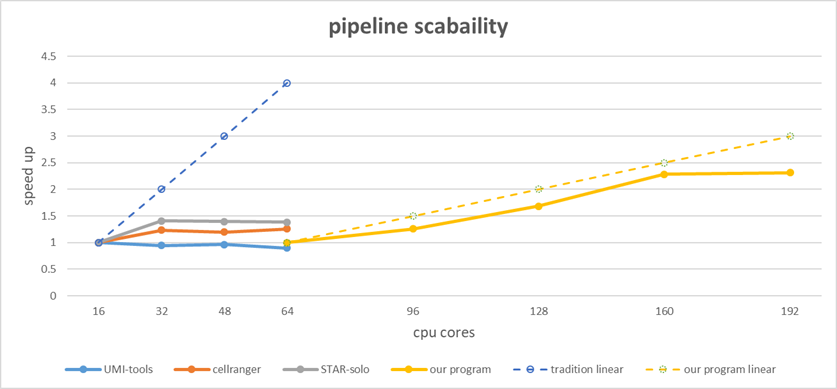
\includegraphics[width=\textwidth]{fig4.png}
  \caption{An overview of Spark version filter.} \label{fig4}
\end{figure}
ScSpark's second advantage is that it can get near linear improvement when the cluster's CPU core number improve.
To test the scalability of the tradition pipeline and scSpark, we use 16 CPU cores performance as tradition pipeline's baseline and 64 CPU cores performance as scSpark's baseline.
We use a small sample which have 100 millions records to compare speedup between our program and tradition pipeline.
As shown in Fig~\ref{fig5}, We found when CPU cores number increase our program can get near linear speedup and tradition pipeline's speedup far below linear speedup.
And we also found if the CPU cores number exceeds a ceiling, both tradition pipeline and scSpark will speedup nearly stop.
Umi-tools isn't showing any scalabiliy, even a little slow down when the CPU cores number increase.
STARsolo and CellRanger shows a little improve when the CPU cores increases to 32 from 16, but quickly stop speedup.
But scSpark ceiling is much higher than tradition pipeline.
All of it explain that our program more scalability than all tradition pipeline.
\subsection{Comparsion each step performance's increase}
\begin{figure}
  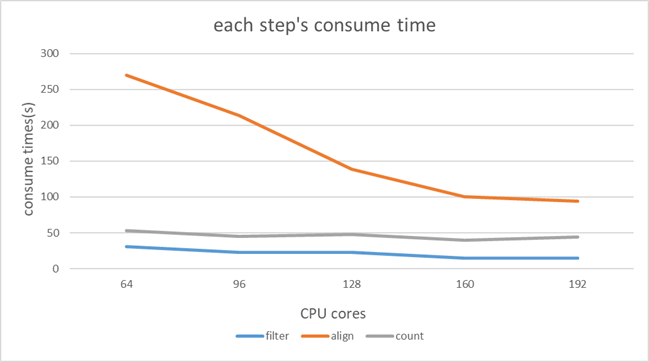
\includegraphics[width=\textwidth]{fig5.png}
  \caption{Each step consumes time.} \label{fig5}
\end{figure}
We also record each step's process time to know the reason of our improve and where can improve in future.
As shown in Fig~\ref{fig5}, we found our program's scalability most come from the align step and the align consumes most time in the whole program.
To find the reason why the align step is more scalability than the other step and why the scalability have a ceiling, we count how much records scSpark's STAR program can process.
We can find in Fig~\ref{fig6}, STAR's mapping speed is influenced by the data volume size and small volume dataset will lost its scalability earier than large volume dataset.
\begin{figure}
  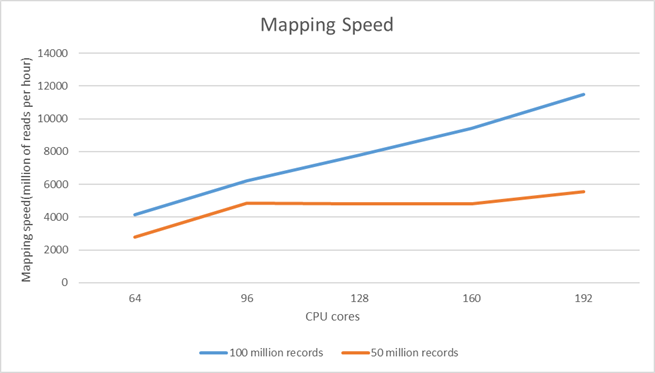
\includegraphics[width=\textwidth]{fig6.png}
  \caption{Invoked STAR's mapping step.} \label{fig6}
\end{figure}

\begin{table}
  \centering
  \caption{Data volume influence}\label{tab3}
  \begin{tabular}{l | l | l | l | l}
  \hline
  Data volume(Million reads) & 10 & 50 & 100 & 640 \\
  \hline
  mapping speed(Million of reads per hour) & 250.28 & 503.83 & 503.02 & 950 \\
  \hline
  \end{tabular}
\end{table}

Then we test STAR program, and find the mapping speed is influenced by data volume.
As Table~\ref{tab3} shown, STAR mapping speed will increase when the data volume increase.
So when we get scalability by increase partition, each partition's read number decrease will limit the scalability increase.

\subsection{Performance Analysis}
We tested performance to find bottleneck of our scSpark.
We used 640 millions records of FASTQ data to evaluate two aspect of our scSpark.
First we compared scSpark spend in network shuffle, disk access and compute time proportion to find whether network shuffle or disk access occupies too much time.
Second we tested CPU and memory usage, to ensure which resources will be scSpark's bottleneck.

\subsubsection{Network and Disk Behavior of scSpark}
\begin{figure}
  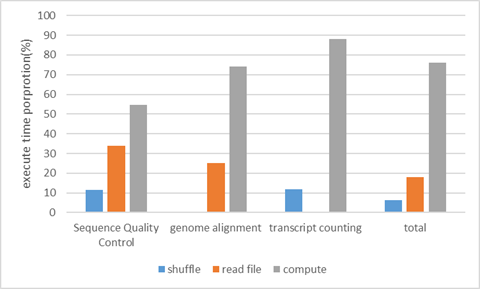
\includegraphics[width=\textwidth]{fig7.png}
  \caption{Each step consumes time.} \label{fig7}
\end{figure}
We computed network time by summing up the time that our scSpark shuffle data in multi machine.
Disk access comes from loading FASTQ, STAR's index and GTF files.
The ideal situation is tasks did not waste any time in disk access and network shuffle.
We found that scSpark's computing time occupies most execute time.
Except STAR's index file, all file's disk access distribute to each node that improve whole system's loading speed.
And we found the time that waste in shuffling doesn't occypy too much time.

\subsubsection{CPU and Memory usage of scSpark}
\begin{figure}
  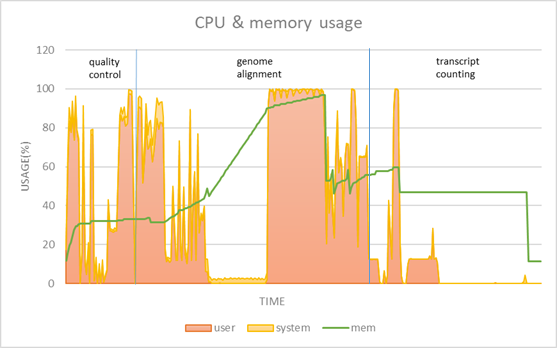
\includegraphics[width=\textwidth]{fig8.png}
  \caption{CPU and Memory usage of scSpark.} \label{fig8}
\end{figure}
We monitored scSpark's CPU and memory usage during processing.
As Fig~\ref{fig8} shown, in sequence quality control step, scSpark highly exploited each node's multi cores CPU to achieve speedup.
Convenition pipelines single thread solution's CPU usage is much lower than scSpark.
And we found that scSpark's boundary much comes from genome alignment.
Because we invoked STAR as our alignment tool, and STAR's program naturally occupy most proportion of memory in this step.
\section{Conclusion}
In this paper, we proposed a way which utilize Apache Spark's in memory compute trait and get considerable speedup and scalability.
Our scSpark can take advantage of multi machine compute capacity to speedup all step and eliminate redundant disk access.

Except performance improve, our scSpark also shows much more scalability than any tradition pipeline which closes to linear improve.
Our scSpark not only can imporve each partition process STAR program's mapping speed, but also can improve scalabliity by increasing partition number if the resource is sufficient.

And we also found our scSpark's scalability improve has a ceiling.
The reason is that our scSpark invokes STAR's mapping speed influenced by loading index time.
And if data volume is tiny, the influence occupies a large proportion of whole the STAR program process time.

\begin{thebibliography}{8}

%\bibliographystyle{splncs04}
%\bibliography{referenceTest}

\bibitem{Papalexi2018SinglecellRS}
Papalexi, E., Satija, R.: Single-cell rna sequencing to explore immune cell
heterogeneity. Nature Reviews Immunology  \textbf{18},  35--45 (2018)

\bibitem{Klein2015DropletBF}
Klein, A.M., Mazutis, L., Akartuna, I., Tallapragada, N., Veres, A., Li, V.,
Peshkin, L., Weitz, D., Kirschner, M.: Droplet barcoding for single-cell
transcriptomics applied to embryonic stem cells. Cell  \textbf{161},
1187--1201 (2015)
  
\bibitem{Macosko2015HighlyPG}
Macosko, E.Z., Basu, A., Satija, R., Nemesh, J., Shekhar, K., Goldman, M.,
Tirosh, I., Bialas, A., Kamitaki, N., Martersteck, E.M., Trombetta, J.J.,
Weitz, D., Sanes, J., Shalek, A., Regev, A., McCarroll, S.: Highly parallel
genome-wide expression profiling of individual cells using nanoliter
droplets. Cell  \textbf{161},  1202--1214 (2015)

\bibitem{tian2018scPipe}
Tian, L., Su, S., Dong, X., Amannzalcenstein, D., Biben, C., Seidi, A., Hilton,
D.J., Naik, S.H., Ritchie, M.E.: scpipe: A flexible r/bioconductor
preprocessing pipeline for single-cell rna-sequencing data. Plos One
\textbf{13}(7),  e0200193 (2018)

\bibitem{Kivioja2012Counting}
Kivioja, T., V?H?Rautio, A., Karlsson, K., Bonke, M., Enge, M., Linnarsson, S.,
Taipale, J.: Counting absolute numbers of molecules using unique molecular
identifiers. Nature Methods  \textbf{9}(1),  72--74 (2012)

\bibitem{camara2017Methods}
Camara, P.G.: Methods and challenges in the analysis of single-cell
rna-sequencing data. Current Opinion in Systems Biology  (2017)

\bibitem{dobin2012RNA}
Dobin, A., Davis, C.A., Schlesinger, F.: Rna-star : ultrafast universal spliced
sequences aligner : Supplementary materials. Hgdownload  (2012)

\bibitem{kim2015hisat}
Kim, D., Langmead, B., Salzberg, S.L.: Hisat: a fast spliced aligner with low
memory requirements. Nature methods  \textbf{12}(4),  357--360 (2015)

\bibitem{smith2017UMI}
Smith, T., Heger, A., Sudbery, I.: Umi-tools: modeling sequencing errors in
unique molecular identifiers to improve quantification accuracy. Genome
research  \textbf{27}(3), ~491 (2017)

\bibitem{swati0zUMIs}
Swati, P., Christoph, Z., Beate, V., Wolfgang, E., Ines, H.: zumis - a fast and
flexible pipeline to process rna sequencing data with umis. Gigaence (6), ~6

\bibitem{zheng2017Massively}
Zheng, G.X.Y., Terry, J.M., Belgrader, P., Ryvkin, P., Bent, Z.W., Wilson, R.,
Ziraldo, S.B., Wheeler, T.D., Mcdermott, G.P., Zhu, J.a.: Massively parallel
digital transcriptional profiling of single cells. Nature Communications
\textbf{8},  14049 (2017)

\bibitem{Svensson2017PowerAO}
Svensson, V., Natarajan, K., Ly, L.H., Miragaia, R., Labalette, C., Macaulay,
I., Cvejic, A., Teichmann, S.: Power analysis of single cell rna-sequencing
experiments. Nature methods  \textbf{14},  381 -- 387 (2017)

\bibitem{Petukhov2018dropEstPF}
Petukhov, V., Guo, J., Baryawno, N., Severe, N., Scadden, D., Samsonova, M.,
Kharchenko, P.: dropest: pipeline for accurate estimation of molecular counts
in droplet-based single-cell rna-seq experiments. Genome Biology  \textbf{19}
(2018)

\bibitem{Smith2017UMItoolsMS}
Smith, T., Heger, A., Sudbery, I.M.: Umi-tools: modeling sequencing errors in
unique molecular identifiers to improve quantification accuracy. Genome
research  \textbf{27 3},  491--499 (2017)

\bibitem{gao2020Comparison}
Gao, M., Ling, M., Tang, X., Wang, S., Xiao, X., Qiao, Y., Yang, W., Yu, R.:
Comparison of high-throughput single-cell rna sequencing data processing
pipelines  (02 2020). \doi{10.1101/2020.02.09.940221}

\bibitem{macosko2015Dropseq}
Macosko, E.Z., Basu, A., Satija, R., Nemesh, J., Shekhar, K., Goldman, M.,
Tirosh, I., Bialas, A.R., Kamitaki, N., Martersteck, E.M., Trombetta, J.J.,
Weitz, D.A., Sanes, J.R., Shalek, A.K., Regev, A., McCarroll, S.A.: Highly
parallel genome-wide expression profiling of individual cells using nanoliter
droplets. Cell  \textbf{161}(5),  1202—1214 (May 2015).
\doi{10.1016/j.cell.2015.05.002},
\url{https://europepmc.org/articles/PMC4481139}

\bibitem{macaulay0Svensson}
Svensson, V., Natarajan, K.N., Ly, L.H., Miragaia, R.J., Labalette, C.,
Macaulay, I.C., Cvejic, A., Teichmann, S.A.: Power analysis of single-cell
rna-sequencing experiments. Nature Methods

\bibitem{viktor2018dropEst}
Viktor, P., Jimin, G., Ninib, B., Nicolas, S., Scadden, D.T., Samsonova, M.G.,Kharchenko, P.V.: dropest: pipeline for accurate estimation of molecular
  counts in droplet-based single-cell rna-seq experiments. Genome Biology
\textbf{19}(1), ~78 (2018)

\bibitem{ref_url1}
UMI\_tools, \url{https://github.com/CGATOxford/UMI-tools}. Last accessed 30
Nov 2020

\bibitem{2019STARsolo}
Blibaum~A, W.J., A., D.: Starsolo: single-cell rna-seq analyses beyond gene
expression [version 1; not peer reviewed]. Genome Informatics  (2019)

\bibitem{ref_url2}
Apache Hadoop framework, \url{https://hadoop.apache.org}. Last accessed 30
Nov 2020

\bibitem{ref_url3}
Apache Spark framework, \url{https://spark.apache.org/}. Last accessed 30
Nov 2020

\bibitem{dean2008mapreduce}
Dean, J., Ghemawat, S.: Mapreduce: simplified data processing on large
clusters. Communications of the ACM  \textbf{51}(1),  107--113 (2008)

\bibitem{zaharia2012resilient}
Zaharia, M., Chowdhury, M., Das, T., Dave, A., Ma, J., McCauly, M., Franklin,
M.J., Shenker, S., Stoica, I.: Resilient distributed datasets: A
fault-tolerant abstraction for in-memory cluster computing. In: Presented as
part of the 9th $\{$USENIX$\}$ Symposium on Networked Systems Design and
Implementation ($\{$NSDI$\}$ 12). pp. 15--28 (2012)

\bibitem{abuin2016sparkbwa}
Abu{\'\i}n, J.M., Pichel, J.C., Pena, T.F., Amigo, J.: Sparkbwa: speeding up
the alignment of high-throughput dna sequencing data. PloS one
\textbf{11}(5),  e0155461 (2016)

\bibitem{li2018high}
Li, X., Tan, G., Wang, B., Sun, N.: High-performance genomic analysis framework
with in-memory computing. ACM SIGPLAN Notices  \textbf{53}(1),  317--328
(2018)

\bibitem{Yang2016Falco}
Yang, A., Michael, T., Lin, P., Ho, J.W.K.: Falco: a quick and flexible
single-cell rna-seq processing framework on the cloud. Bioinformatics (5), ~5
(2016)

\bibitem{ref_url4}
10xgenomics, \url{https://support.10xgenomics.com}. Last accessed 30
Nov 2020

\bibitem{ref_url5}
Index and GTF file, \url{https://www.gencodegenes.org/human/releases.html}. Last accessed 30
Nov 2020

\bibitem{divya2013elasticsearch}
Divya, M.S., Goyal, S.K.: Elasticsearch: An advanced and quick search technique
to handle voluminous data. Compusoft  \textbf{2}(6), ~171 (2013)

\end{thebibliography}
\end{document}
